\documentclass[12pt,a4paper,oneside]{article}

\usepackage[utf8]{inputenc}
\usepackage[T1]{fontenc}
\usepackage[french]{babel}
\usepackage{amssymb}
\usepackage{amsmath}
\usepackage{graphicx}
\usepackage{float}


\author{Matteo Besançon}
\title {Préparation examens outils formels}
\date{\today}
\begin{document}
	\maketitle

\section{Formalisme RdP}
	\subsubsection*{1. Définition formelle de la structure des RdP (syntaxe)}
		\begin{description}
			\item [P] Places (Rond)
			\item [T] Transitions (Rectangle)
			\item [ ] Jeton (point noir)
			\item [$M_0$] Marquage initial
			\item [$M_n$] Marquage après la n ième transition
		\end{description}

		Un réseau R est un quadruplet R

		$$R = (P,T, Entree, Sortie)$$

		Pour $p \in P$ et $t \in T$ si :
		\begin{itemize}
			\item $k = Entree(p,t) > 0$ $p$ est une place d'entrée de $t$ et $t$ est une place de sortie de $p$
			\item $k = Sortie(p,t) > 0$ $p$ est une place de sortie de $t$ et $t$ est une place d'entrée de $p$
		\end{itemize}

		On a les représentations matricielles suivantes :

		\begin{figure}[H]
			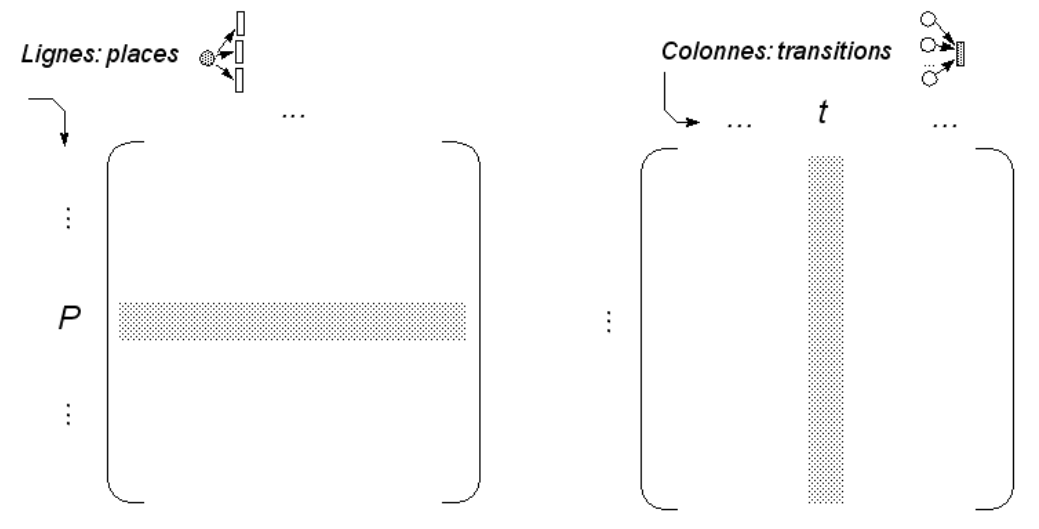
\includegraphics[scale = 0.4]{./img/entree.png}
			\centering
			\caption{Matrice d'entrée et de sortie}
			\label{entreeSortie}
		\end{figure}

		Par exemple avec le RdP suivant :

		\begin{figure}[h]
			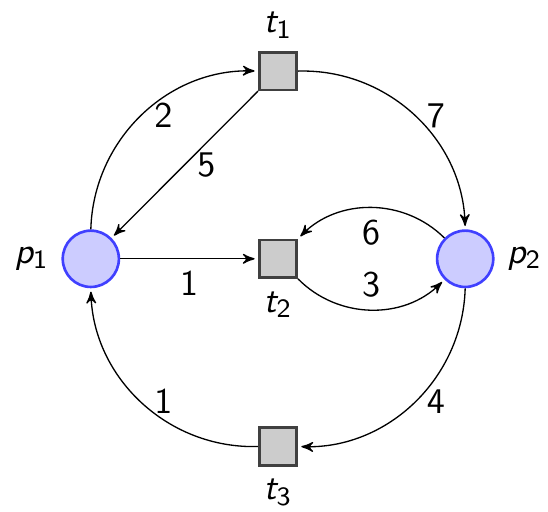
\includegraphics[scale = 0.5]{./img/exrdp.png}
			\centering
			\caption{RdP d'exemple}
		\end{figure}

		On a donc les matrices suivantes :
		$$Entree = \begin{bmatrix}
			2 & 1 & 0 \\
			0 & 6 & 4
		\end{bmatrix}
		Sortie = \begin{bmatrix}
			5 & 0 & 1 \\
			7 & 2 & 0
		\end{bmatrix}$$


	\subsubsection*{2. Définition formelle des règles de franchissabilité des transitions (sémantique)}
		Y a un jeton et paf plus de jeton !!

	\subsubsection*{3. Utilisation de l’algèbre linéaire pour définir la franchissabilité des transitions}





\end{document}
